\documentclass[UTF8]{ctexart}
\usepackage{graphicx}
\title{基于RaspberryPi的厕所空气质量智能在线监管系统 立项建议书}
\author{陈彦宁, 刘涵之}
\date{2019 年 10 月 10 日}
\begin{document}
\maketitle
\pagebreak
\tableofcontents
\pagebreak
\section{发现问题}
在宿舍生活中我们发现,没有安装排风系统的寝室厕所(蹲便器)在每次如厕后的很长一段时间内都会有一股难以去除的异味,异味散发到寝室内部,直接影响了整个寝室的空气质量情况,给我们带来了极大的困扰。若是能设计一种系统,可以动态感知异味气体的浓度,智能主动式除臭,就可以很大程度上解决由寝室厕所引发的寝室异味问题。
\section{解决方案}
制作一种基于RaspberryPi的在线异味监管系统(BrownSense),其中RaspberryPi采用 5V 2A MicroUSB供电,除臭系统采用12V直流供电,面向用户的在线系统使用web实现。通过RaspberryPi(终端设备)实现异味气体浓度的实时获取与云端上传,并实现获取云端的除臭指令后控制继电器开关从而进行主动式除臭流程。对于在线系统,数据后端管理所有的终端设备,记录、分析数据并发送各类控制指令。监控前端上实时显示所有终端设备的状态,监控所有厕所的异味气体浓度情况,并展现所有终端设备记录的异味气体浓度图表与除臭运作状态,并在发生异常或除臭手段开始运作时显示警告。

部署完毕后,用户只需使用任意浏览器打开监控应用,便可一目了然地查看所有厕所的状态。页面上将有一个动态更新的图表,以不同颜色展示各个厕所的状况(气味良好/异常,设备正常/故障,主动除臭是否运行)。当用户指定某一终端,将展示该厕所实时更新的历史气味浓度图表与当前实时变化趋势。用户可在应用中设定主动除臭的气体浓度触发策略以实现自动除臭,或手动强制启动除臭功能以应对突发状况。
\section{可行性分析}
\subsection{系统构成}
系统分为三个部分:终端设备、数据后端与监控前端。终端设备为传感器与执行器的搭载端,通过板载模块实现数据采集与主动空气净化等主体功能。数据后端为中间层,作为网关管理所有的终端设备,记录所有设备的历史数据与状态,同时负责下放各类控制指令。监控前端为面向最终用户的 Web 单页应用,为用户可接触到的界面,使得用户可以查看所有终端设备的状态,监控所有厕所的情况,并允许用户控制系统的运行。

其逻辑架构如图 \ref{fig:diagram} 所示。
\begin{figure}[htbp]
    \noindent\makebox[\textwidth]{
        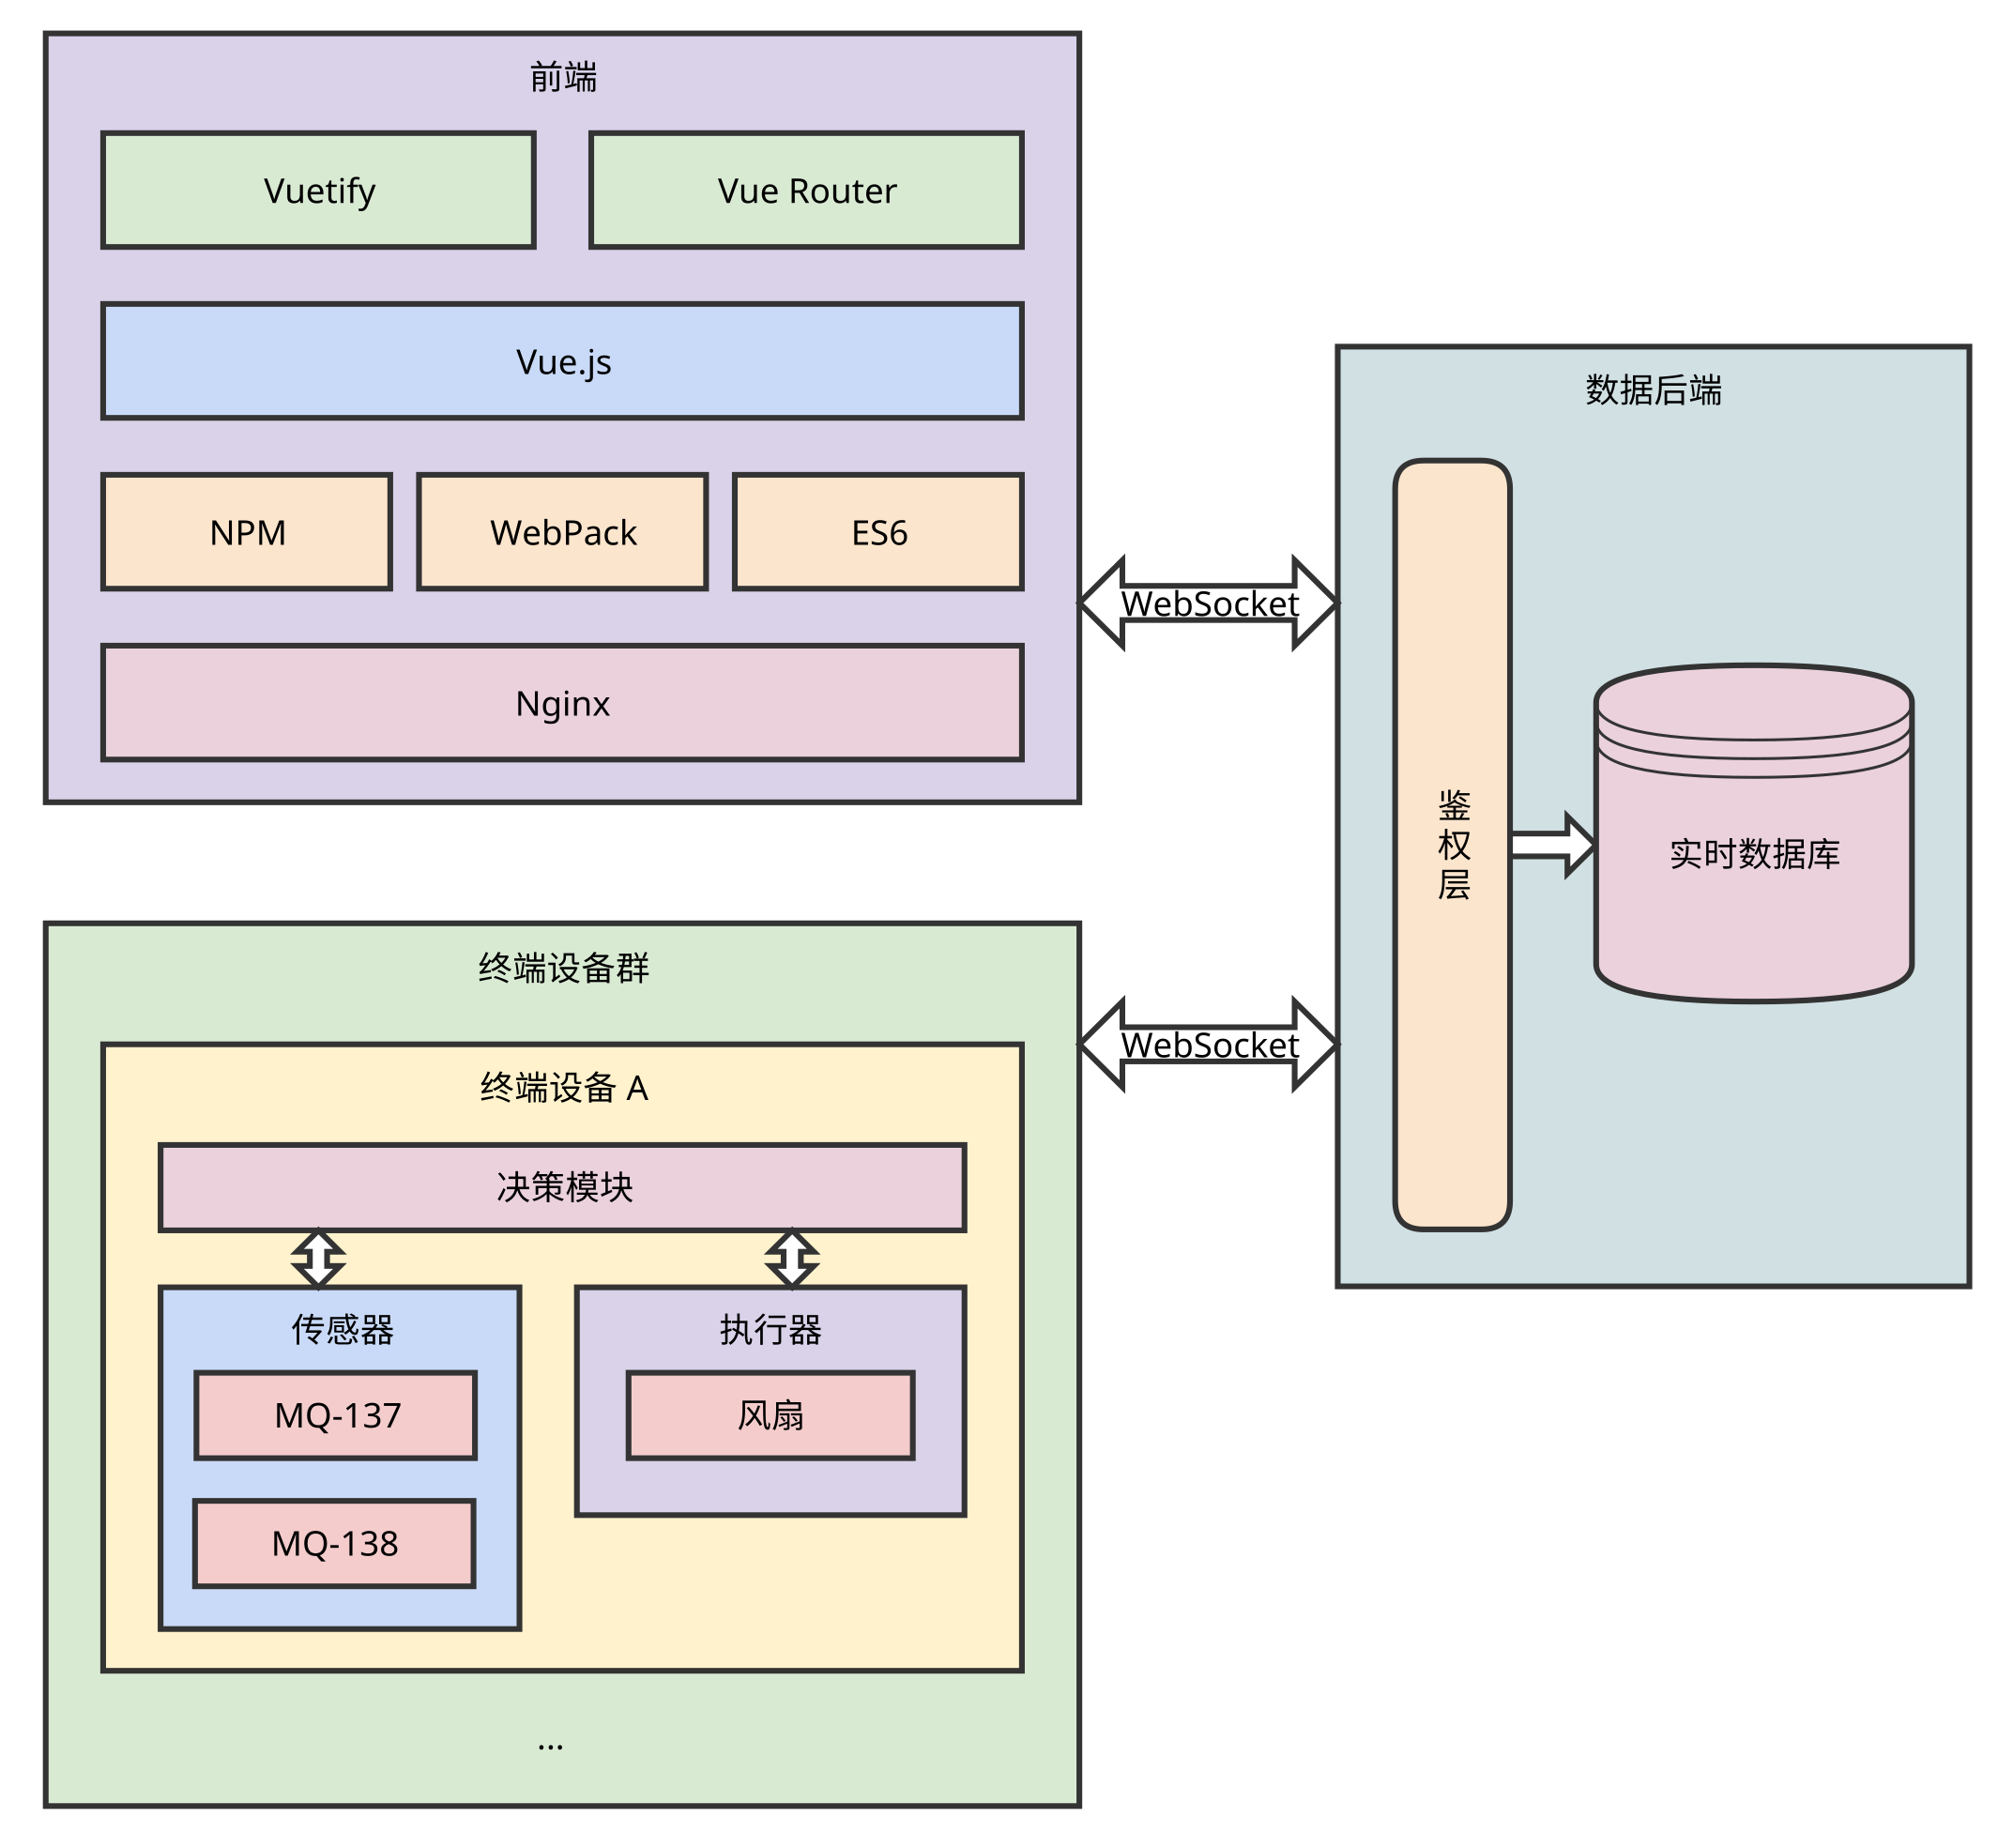
\includegraphics[width=.8\textwidth]{diagram.png}
    }
    \caption{逻辑架构}\label{fig:diagram}
\end{figure}
\subsection{技术选型}
终端设备为树莓派开发版,其上搭载 H2S(g) 与 NH3(g) 传感器,以实现对厕所臭味状况的实时感知。同时,可外接继电器或输出其他信号,以实现智能开启排风扇、喷洒除臭剂等主动防控功能。设备使用 5V 2A MicroUSB 供电,原型将使用充电宝/适配器进行供电,在生产环境可以考虑使用热插拔电池包。设备使用 WiFi 或 4G 网络接入互联网,并拥有自己的设备 token,以实时回传数据。

数据后端的存储部分预计由运行在互联网上的本地实时数据库(Couch\-DB, PouchDB 等)服务器或 Serverless 服务(Firebase, LeanCloud 等)实现,以 WebSocket 协议或 Ajax 请求承载 Json API 完成数据的读写。同时,指令以数据的形式写入数据库并在各端间同步,以实现最好的实时性,并便于权限管理。

监控前端为 Web 单页应用,使用 Vuetify UI 框架与 Vue.js 页面框架,展现所有终端记录的臭味浓度图表与除臭运作状态,并在发生异常或除臭手段开始运作时发出警告。同时,使用双向绑定的 MVVM 模型,数据与图表实时刷新,使过去与当前的厕所气味状态和设备运行状态一目了然,便于监控操作。
\subsection{系统运行}
在初期,用户需在有检测需求的厕所中安装终端设备。设备可以胶水或螺丝等方式固定在墙上等位置,确保电源联通,并完成网络配置(4G 或 WiFi)。

部署完毕后,用户只需使用任意浏览器打开监控应用,便可一目了然地查看所有厕所的状态,并对紧急状况进行干预。页面上将有一个动态更新的图表,以不同颜色展示各个厕所的状况(气味良好/异常,设备正常/故障,主动除臭是否运行)。当用户指定某一终端,将展示该厕所实时更新的历史气味浓度图表与当前实时变化趋势。用户可在应用中设定主动除臭的气体浓度触发策略以实现自动除臭,或手动强制启动除臭功能以应对突发状况。

如果使用电池供电方案,需要在终端发出电量低警告时及时更换电池。
\section{实施计划}
\paragraph{第1周}确定系统整体框架,初步确定实现方案,购买所需硬件设备与云端服务
\paragraph{第2周}配置RaspberryPi及云端环境;编写后端程序,实现后端数据存取、控制操作
\paragraph{第3周}编写前端程序,实现实时数据、图表、除臭系统运行状态更新、查看功能
\paragraph{第4周}完善前端程序,补充实现其他辅助功能;实现后端调控终端除臭系统运行功能
\paragraph{第5周}系统整体运行调试,检查、修复漏洞
\paragraph{第6、7、8周}美化前端页面,系统长时间运行稳定性测试
\section{经费预算}
经费预算见 表 \ref{tab:bom}。
\begin{table}[htbp]
    \noindent\makebox[\textwidth]{
        \begin{tabular}{c|c|c|c}
            \hline
            材料名称             & 单价/元 & 数量 & 总价/元 \\
            \hline
            Raspberry Pi 4B      & 435     & 1    & 435     \\
            \hline
            MQ-137 氨气传感器    & 85      & 1    & 85      \\
            \hline
            MQ-136 硫化氢传感器  & 85      & 1    & 85      \\
            \hline
            BG0903-B049-P0S 风扇 & 20      & 1    & 20      \\
            \hline
            ADC 模块             & 148     & 1    & 148     \\
            \hline
            ECS 服务器           & 120     & 1    & 120     \\
            \hline
            总计                 & ---     & ---  & 893     \\
            \hline
        \end{tabular}
    }
    \caption{经费预算}\label{tab:bom}
\end{table}
\pagebreak
\end{document}
